\usetikzlibrary{arrows.meta, positioning, calc}

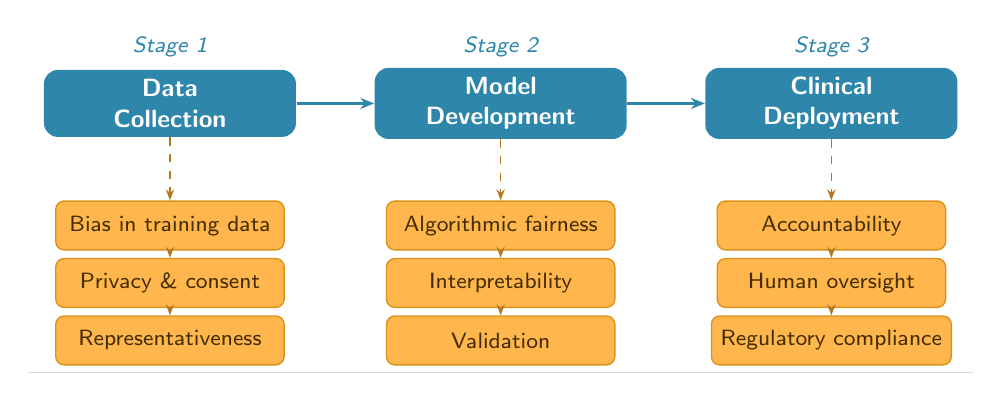
\begin{tikzpicture}[
    every node/.style={font=\small\sffamily},
    main/.style={
        rectangle, rounded corners=5pt,
        fill={rgb,255:red,46;green,134;blue,171},
        text=white,
        minimum width=3.2cm, minimum height=0.85cm,
        align=center, font=\small\sffamily\bfseries
    },
    ann/.style={
        rectangle, rounded corners=3pt,
        fill={rgb,255:red,255;green,183;blue,77},
        text={rgb,255:red,70;green,45;blue,0},
        minimum width=2.9cm, minimum height=0.62cm,
        align=center, font=\footnotesize\sffamily,
        draw={rgb,255:red,220;green,145;blue,25},
        line width=0.5pt
    },
    arr/.style={
        -{Stealth[length=5pt,width=4pt]},
        line width=0.9pt,
        color={rgb,255:red,46;green,134;blue,171}
    },
    dann/.style={
        dashed,
        -{Stealth[length=4pt,width=3pt]},
        line width=0.5pt,
        color={rgb,255:red,180;green,120;blue,30}
    },
    stg/.style={
        font=\footnotesize\sffamily\itshape,
        text={rgb,255:red,46;green,134;blue,171}
    }
]

%% ── Stage labels ────────────────────────────────────────────────────
\node[stg] at (0,   0.72) {Stage 1};
\node[stg] at (4.2, 0.72) {Stage 2};
\node[stg] at (8.4, 0.72) {Stage 3};

%% ── Main pipeline ───────────────────────────────────────────────────
\node[main] (dc) at (0,   0) {Data\\Collection};
\node[main] (md) at (4.2, 0) {Model\\Development};
\node[main] (cd) at (8.4, 0) {Clinical\\Deployment};

\draw[arr] (dc) -- (md);
\draw[arr] (md) -- (cd);

%% ── Annotation boxes: Data Collection ──────────────────────────────
\node[ann] (dc1) at (0.0, -1.55) {Bias in training data};
\node[ann] (dc2) at (0.0, -2.28) {Privacy \& consent};
\node[ann] (dc3) at (0.0, -3.01) {Representativeness};

\draw[dann] (dc.south)  -- (dc1.north);
\draw[dann] (dc1.south) -- (dc2.north);
\draw[dann] (dc2.south) -- (dc3.north);

%% ── Annotation boxes: Model Development ────────────────────────────
\node[ann] (md1) at (4.2, -1.55) {Algorithmic fairness};
\node[ann] (md2) at (4.2, -2.28) {Interpretability};
\node[ann] (md3) at (4.2, -3.01) {Validation};

\draw[dann] (md.south)  -- (md1.north);
\draw[dann] (md1.south) -- (md2.north);
\draw[dann] (md2.south) -- (md3.north);

%% ── Annotation boxes: Clinical Deployment ───────────────────────────
\node[ann] (cd1) at (8.4, -1.55) {Accountability};
\node[ann] (cd2) at (8.4, -2.28) {Human oversight};
\node[ann] (cd3) at (8.4, -3.01) {Regulatory compliance};

\draw[dann] (cd.south)  -- (cd1.north);
\draw[dann] (cd1.south) -- (cd2.north);
\draw[dann] (cd2.south) -- (cd3.north);

%% ── Bottom rule ─────────────────────────────────────────────────────
\draw[gray!30, line width=0.4pt]
    (-1.8, -3.42) -- (10.2, -3.42);

\end{tikzpicture}
